\documentclass[12pt,oneside]{paper}

\usepackage{listings}
\renewcommand{\lstlistingname}{saucecode}

\lstset{%
  language={C},
  basicstyle={\small},%
  identifierstyle={\small},%
  commentstyle={\small\itshape},%
  keywordstyle={\small\bfseries},%
  ndkeywordstyle={\small},%
  stringstyle={\small\ttfamily},
  frame={tb},
  breaklines=true,
  columns=[l]{fullflexible},%
  numbers=left,%
  xrightmargin=0zw,%
  xleftmargin=3zw,%
  numberstyle={\scriptsize},%
  stepnumber=1,
  numbersep=1zw,%
  lineskip=-0.5ex%
}



% タイトル
\title{1軸レーザー距離センサを用いたQudad Rotorの周辺認識についての研究}
\author{高倉啓祐・中野晋}

\begin{document}
% 行間
\setlength{\baselineskip}{9truemm}

%文字間
\kanjiskip=.53zw plus 3pt minus 3pt
\xkanjiskip=.53zw plus 3pt minus 3pt

% 目次
\tableofcontents
%\newpage

% 本文
\chapter{はじめに}

\section{研究の背景}
当研究室では例年,高専ロボコンに出場するためのロボットを設計・製作を行っている.今年度はプラ段ボールを如何に高く積み上げるかを競うための積込ロボットの製作を行った.この積み込みロボットにはリフトが搭載されており(図\ref{fig:robot}),このリフトが上下することでプラ段ボールの箱を持ち上げたり降ろすことが出来る.リフトには上端と下端にリミットセンサが設置されており,その位置でリフトが停止するようになっている.しかし,リミットセンサによる位置検出では,センサのある場所にしかリフトを停止させることが出来ない.任意の高さで停止させるには位置を連続的に検出できるセンサを使用した位置制御が必要になるが,そのようなセンサの使用にはコストがかかる.そこで,コストのかかるセンサを使用せずに位置制御を行う方法はないかと考えた.

\begin{figure}[htbp]
  \begin{center}
    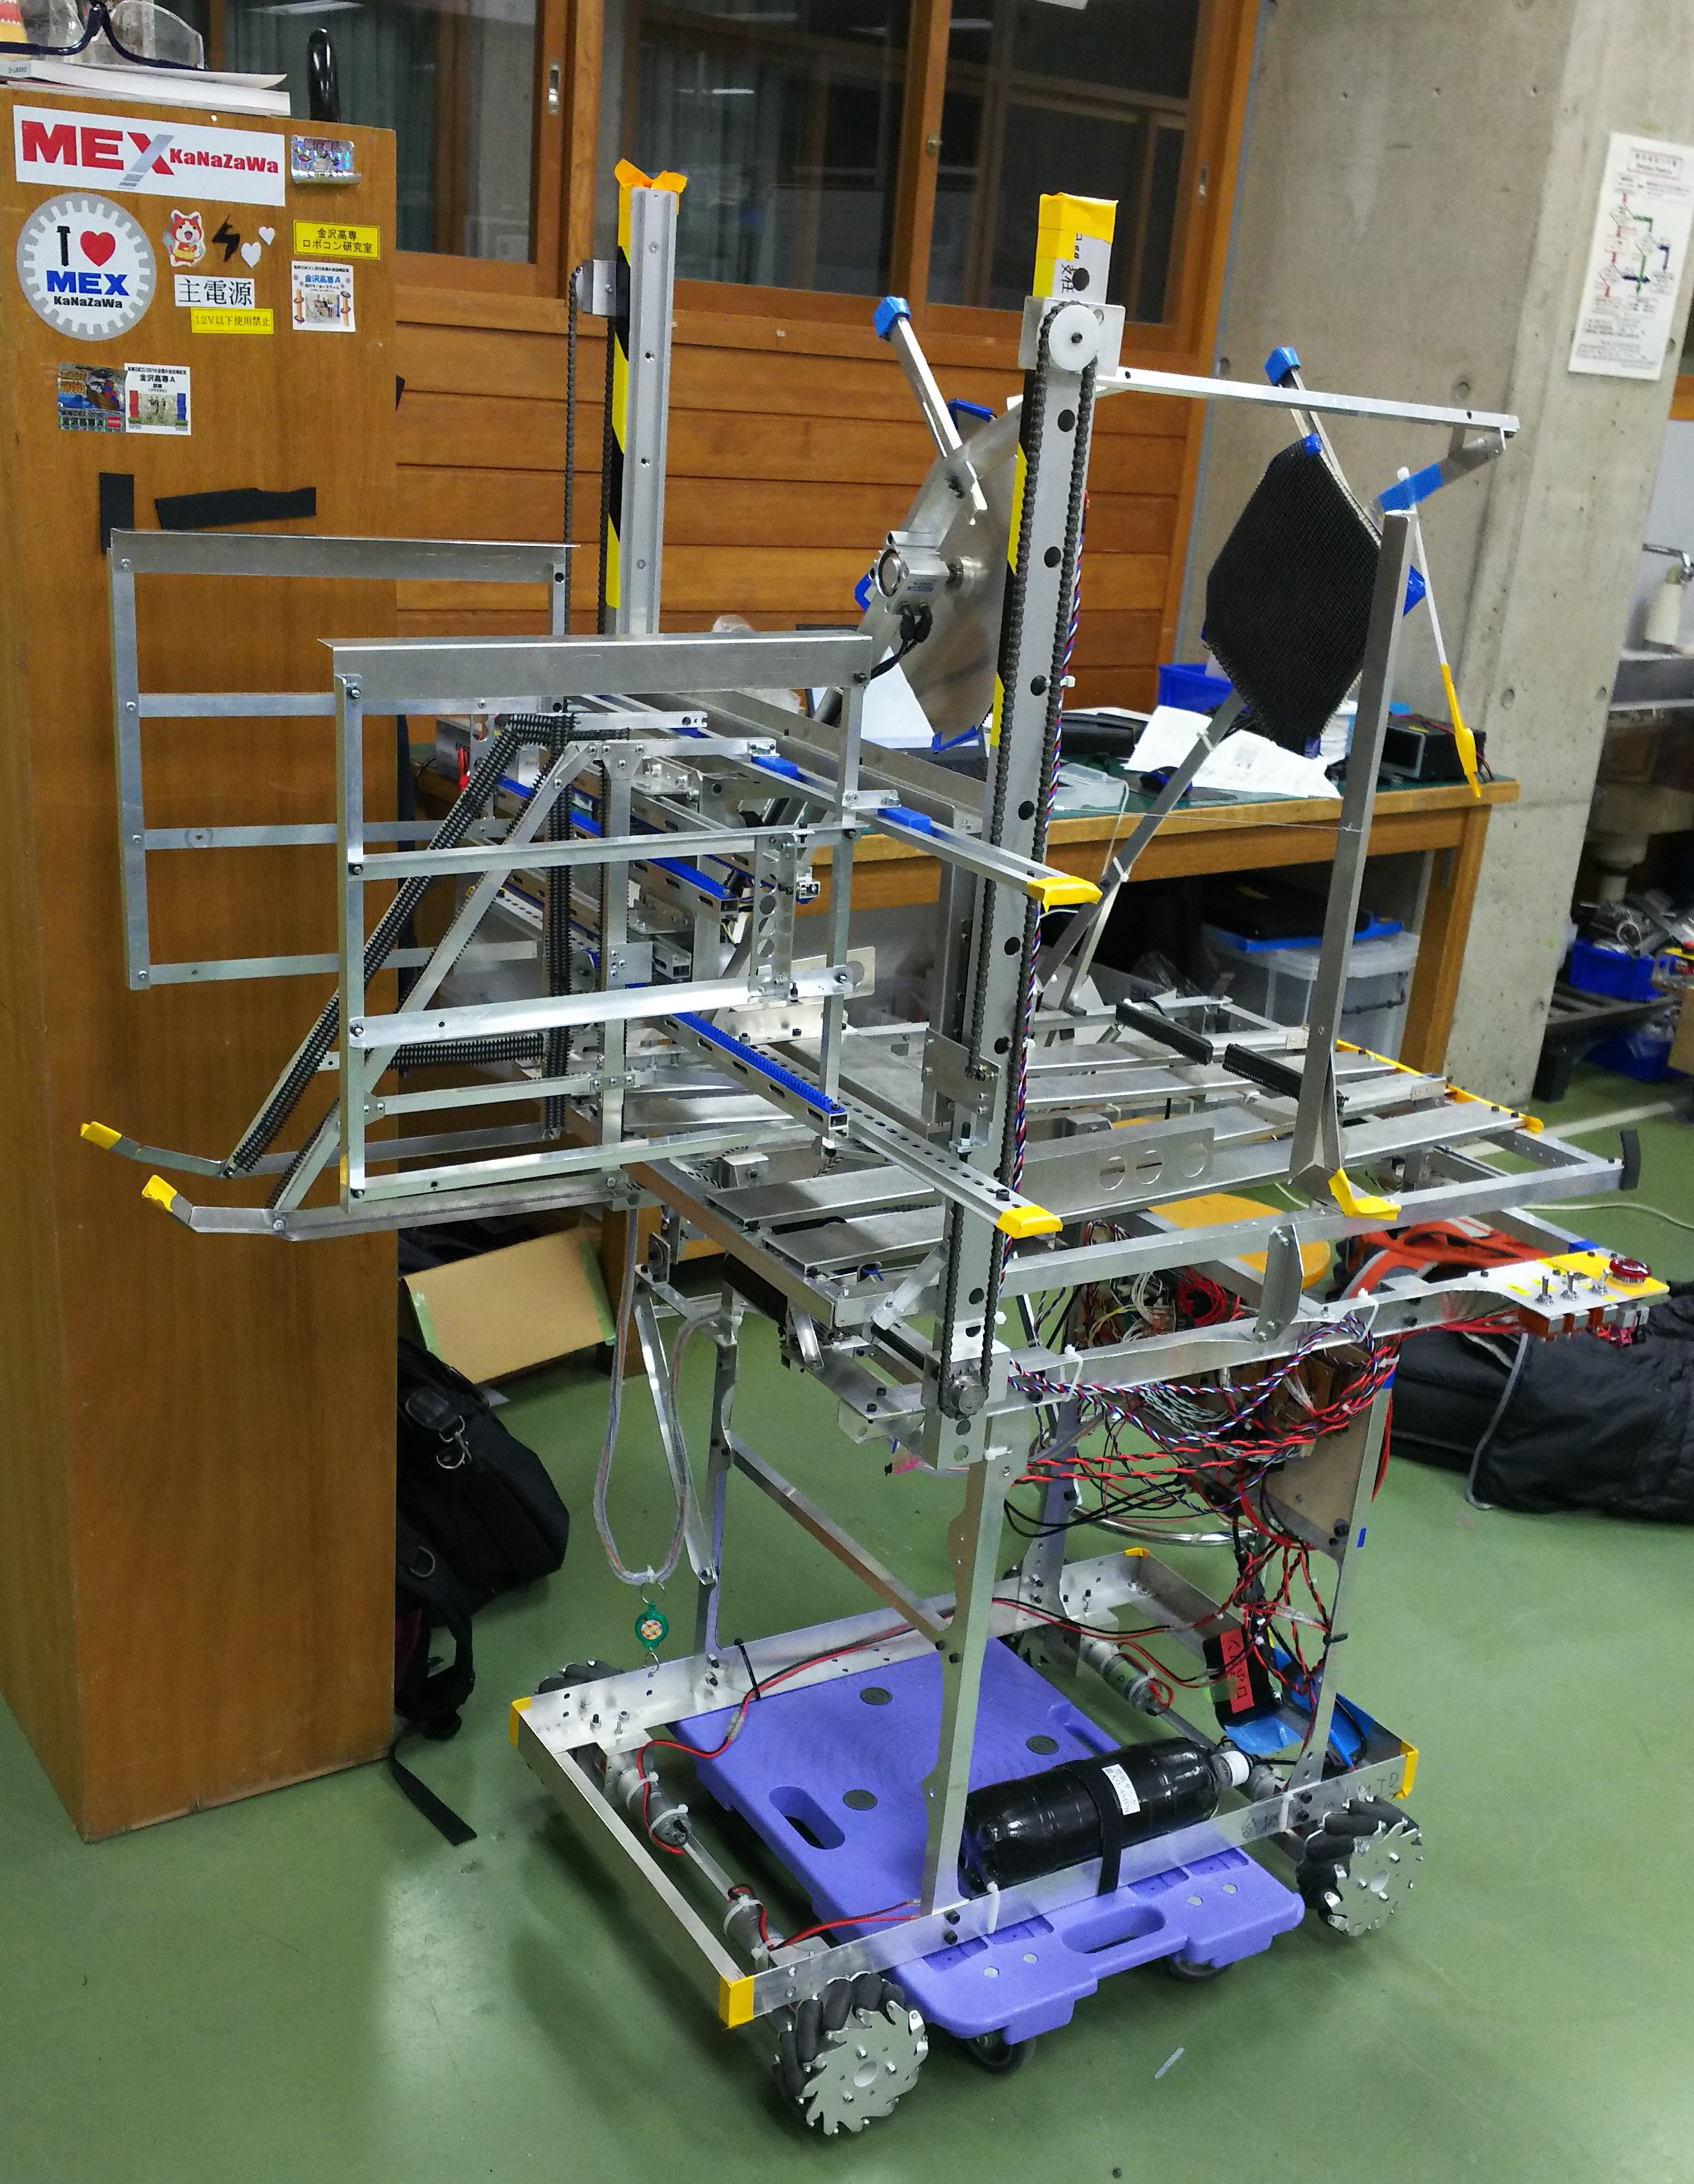
\includegraphics[width=80mm]{img/robot.JPG}
    \end{center}
  \caption{積み込みロボット}
 \label{fig:robot}
\end{figure}

\section{研究の目的}
ロータリーエンコーダやポテンショメータといった,直接リフトの位置を検出できるセンサを使用することなく,リフトを任意の位置に停止させる制御を考案する.


\section{本論文の構成}
1章では,本研究の背景と簡略化した概要を示す.2章では製作したリフトについて,高専ロボコンのルールをからめつつ述べる.3章では通常用いられる位置制御について述べる.4章では位置センサを使用しない制御の手法について述べる.5章ではシミュレーションソフトを用いた実験を示す.6章で最後に本実験のまとめを述べる.

\chapter{リフトについて}

\section{要求される仕様}
\subsection{ロボコンのルール}
今年度のロボコンのタイトルは「ロボット・ニューフロンティア」で,新大陸の開拓をテーマとしている.今回の競技フィールドを(図\ref{fig:field})に示す.新大陸では,スタート地点から運んできたプラスティック製段ボールの箱(図\ref{fig:plabox})を高く積み上げる課題が課されている.港町と島,島と新大陸までの間の海にはロボットは接地してはならない.積み上げロボットはスタート地点と島に置いてあるプラスティック製段ボールを取りに行き高台に小さい砦を積み上げる.高台の砦が完成後,新大陸に向かい丘に砦を完成させる.これを2チームでいかに高く積み上げるかを競い合う競技となっている.

\begin{figure}[htbp]
  \begin{center}
    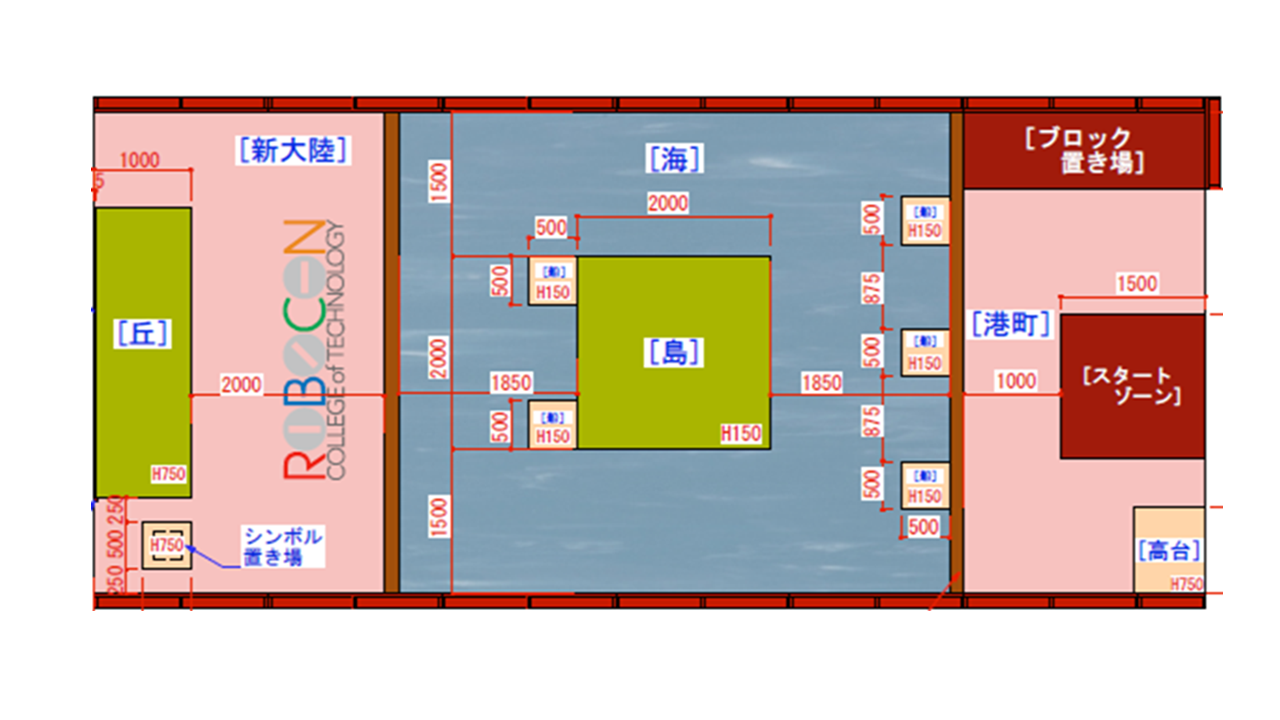
\includegraphics[width=130mm]{img/field.png}
    \end{center}
  \caption{競技フィールド}
 \label{fig:field}
\end{figure}

\subsection{我々の戦略}
プラスティック製段ボールの積み方を(図\ref{fig:tumikata})に示すように,同じ数の箱を積み上げる場合,箱の長手方向を縦向きにして積み上げる方が高く積み上げられる.よってリフトの可動高さを400[mm]になるよう設計,製作した.だが,長手方向を縦向きにすることで重心位置が高くなり,底面積が減るため落下時にバランスが崩れ,倒れる恐れがあるため注意する必要がある.


\begin{figure}[htbp]
  \begin{center}
    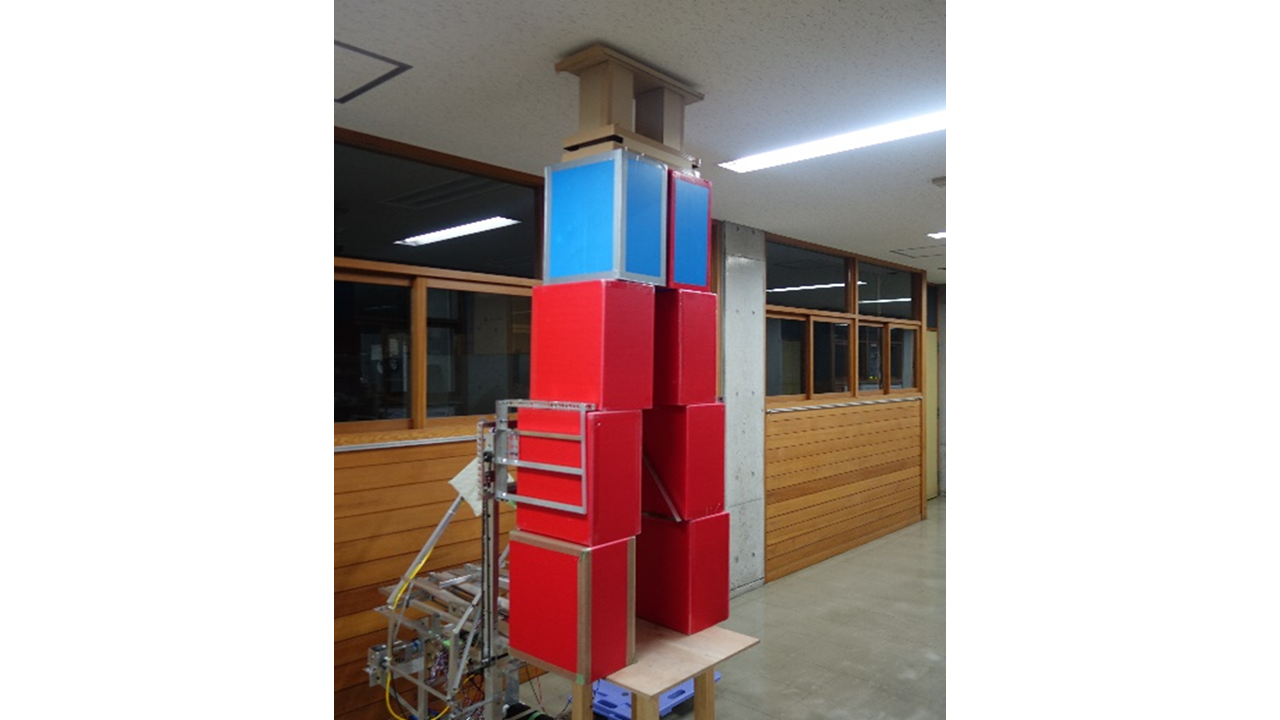
\includegraphics[width=90mm]{img/tumikata.png}
    \end{center}
  \caption{プラスティック段ボールの積み方}
 \label{fig:tumikata}
\end{figure}

\begin{figure}[htbp]
  \begin{center}
    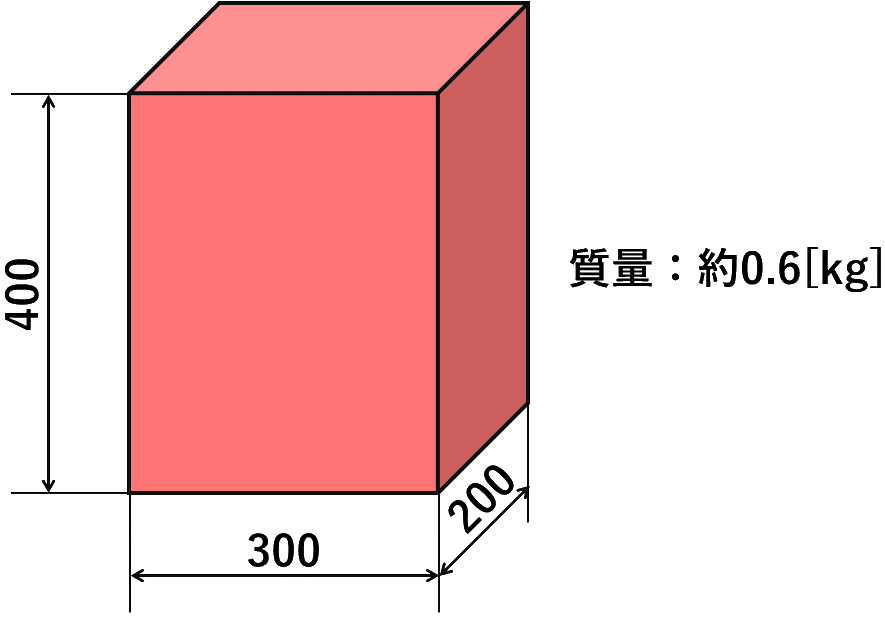
\includegraphics[width=100mm]{img/plabox.png}
    \end{center}
  \caption{プラ段の箱の仕様}
 \label{fig:plabox}
\end{figure}




\section{動作原理}
積込ロボットの前面にリフトが搭載されている(図\ref{fig:lift}).
リフト中央下部に設置されているモータによってスプロケットが回転し,チェーン駆動をする.
リフト上端と下端に設置してあるリミットセンサには通過型フォトインタラプタを使用している.リミットセンサは距離が400[mm]になるように位置が調整されているため,箱を400[mm]の高さに持ち上げることが出来る.



\begin{figure}[htbp]
  \begin{center}
    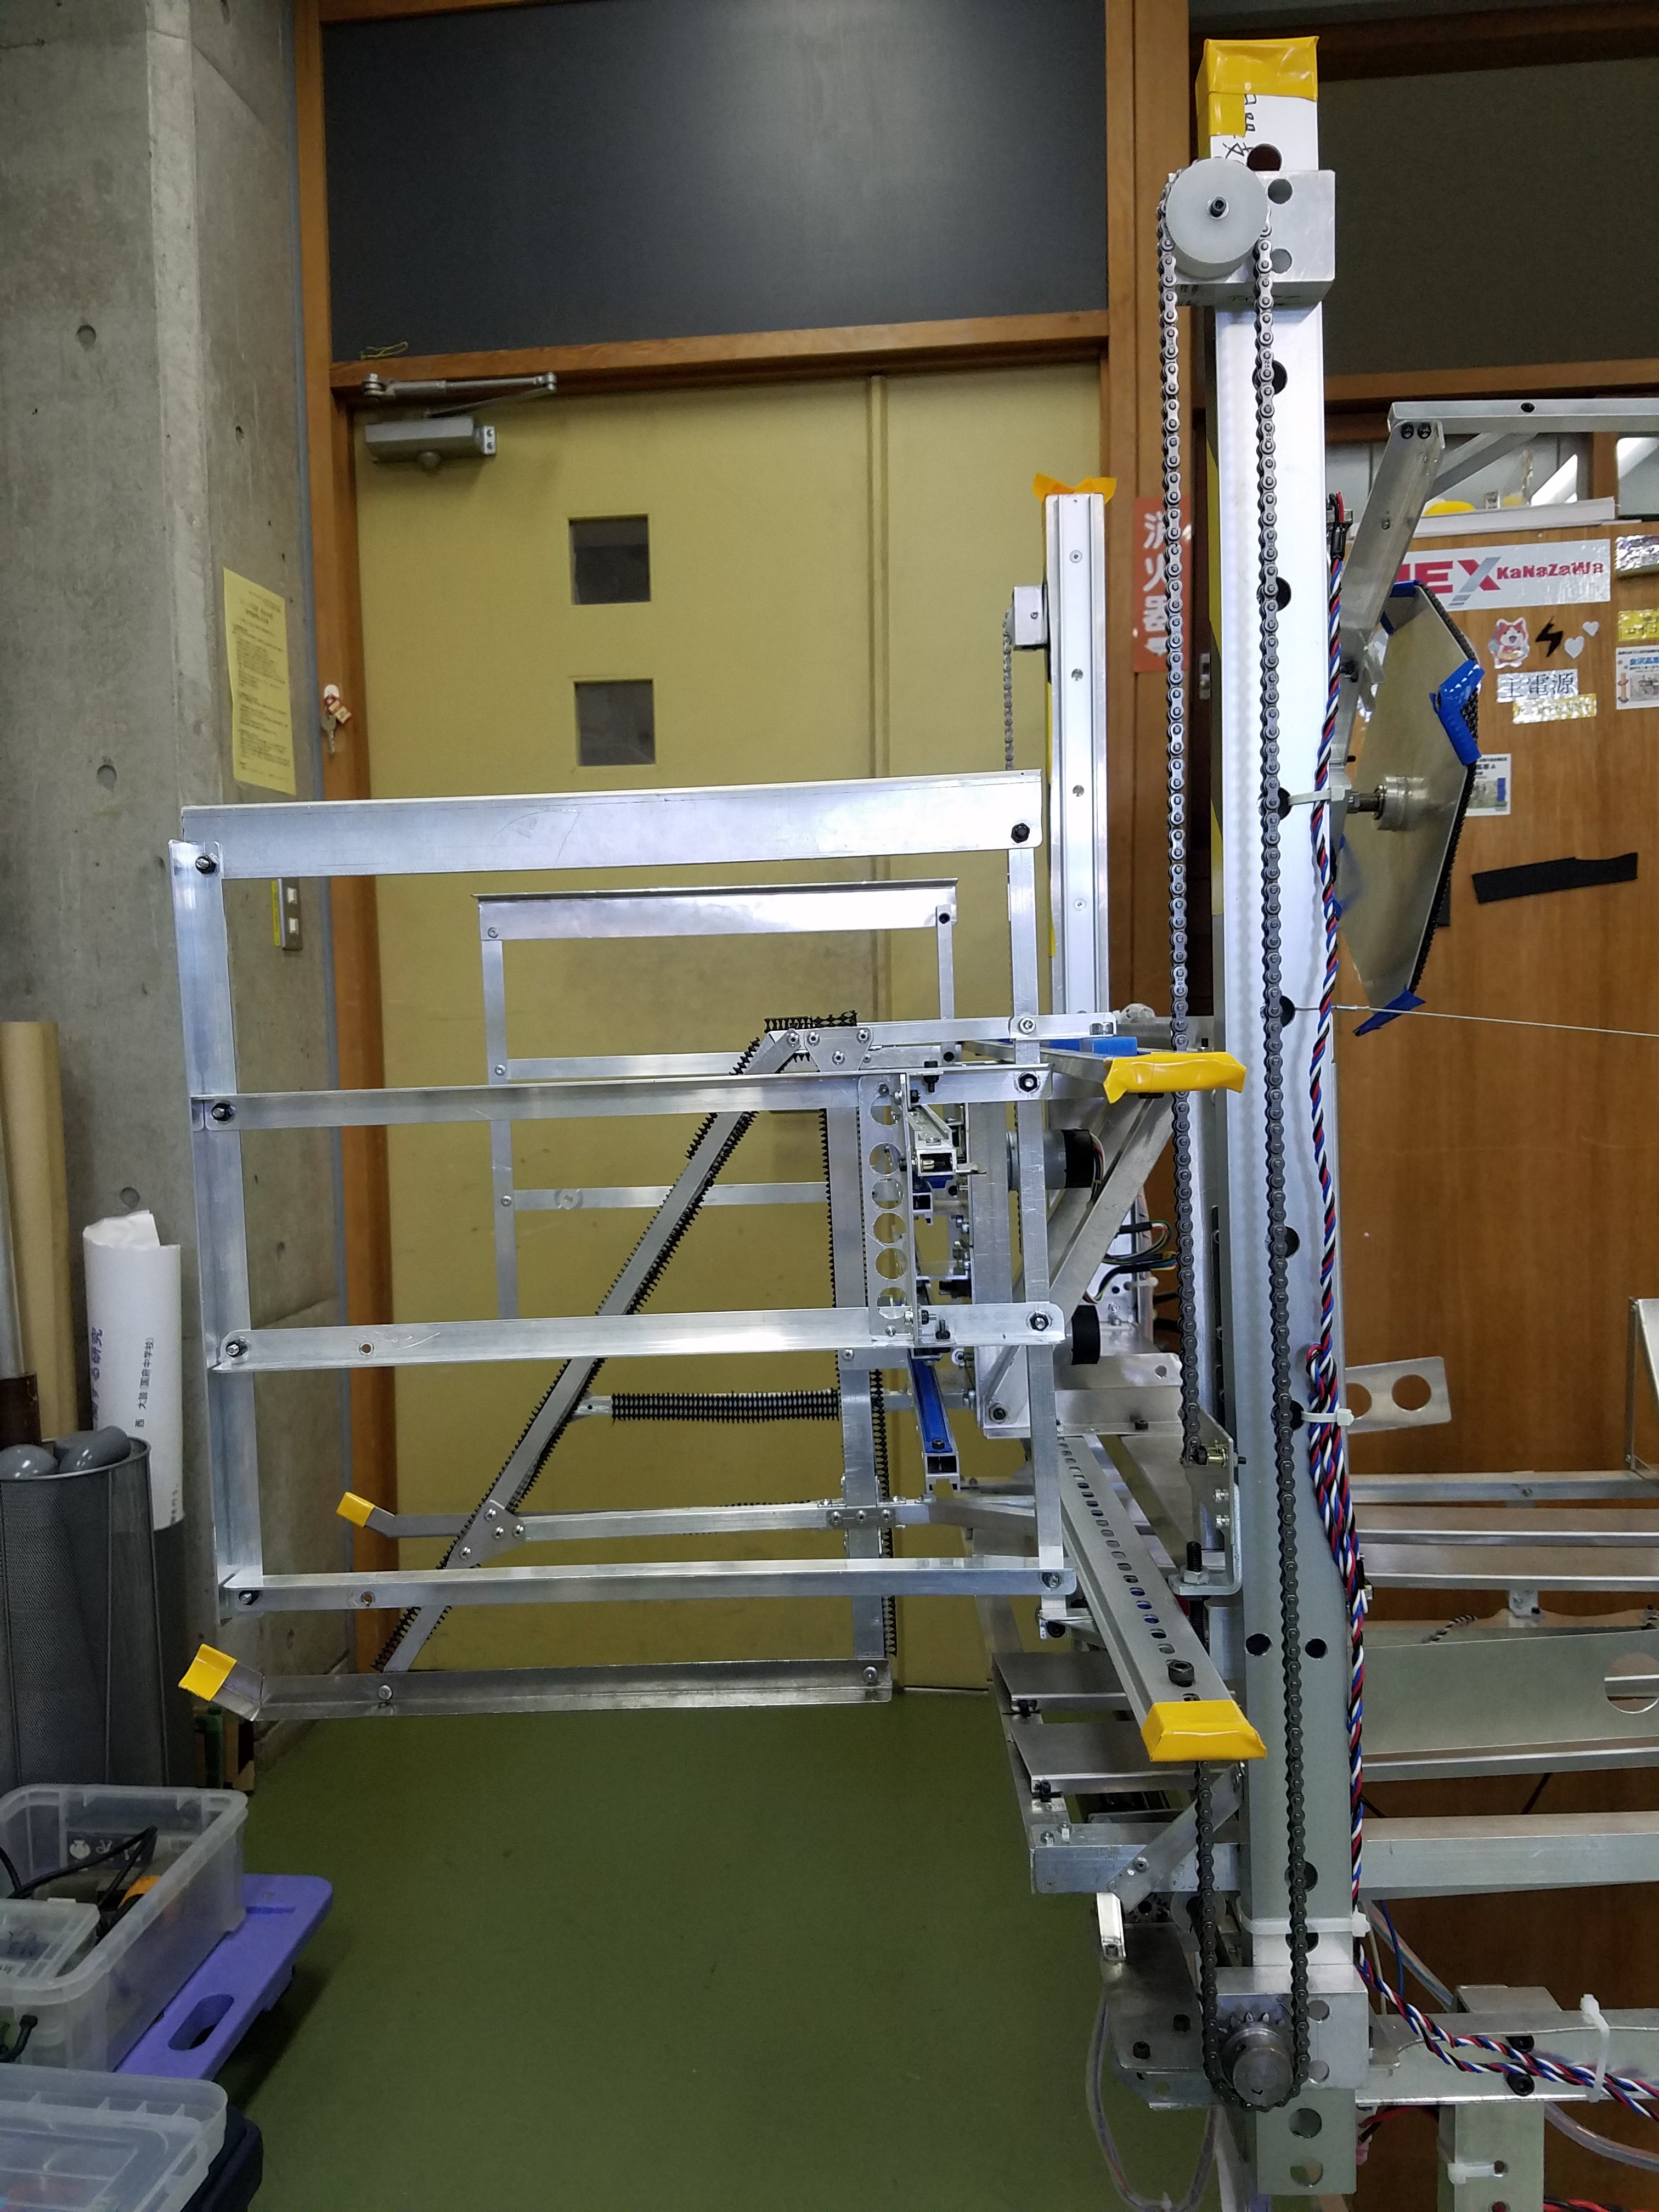
\includegraphics[width=80mm]{img/lift.jpg}
    \end{center}
  \caption{積み込みロボットのリフト}
 \label{fig:lift}
\end{figure}

\section{回路構造}
リフトに関わるロボットのシステムブロック線図は図\ref{fig:roboblock}のようになっている.arduinoは図\ref{fig:arduino}にあるようなarduinoMegaを使用した.このarduinoはUSBホストシールド(図\ref{fig:USBhs})を介したBluetoothでの通信でコントローラの信号を受け取る.コントローラでの操作と上下リミットセンサの信号を受け取り,図\ref{fig:motordrive}のモータドライバに指示を送り,リフト駆動用のモータを制御している.モータドライバはarduinoから正転,逆転,PWM値を受け取り,モータに最大12[V]の電圧を印加する.

\begin{figure}[htbp]
  \begin{center}
    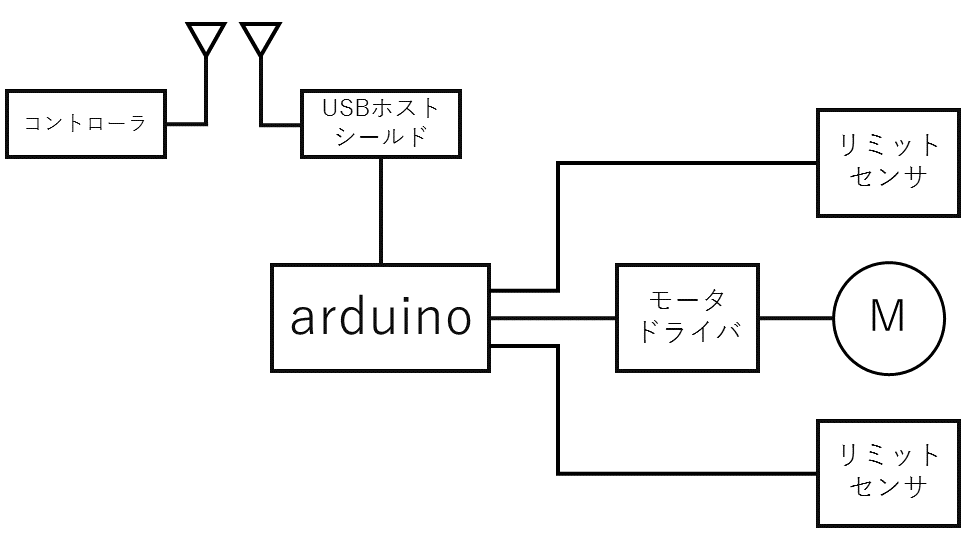
\includegraphics[width=120mm]{img/roboblock.png}
    \end{center}
  \caption{ロボットのシステムブロック線図}
 \label{fig:roboblock}
\end{figure}

\begin{figure}[htbp]
  \begin{center}
    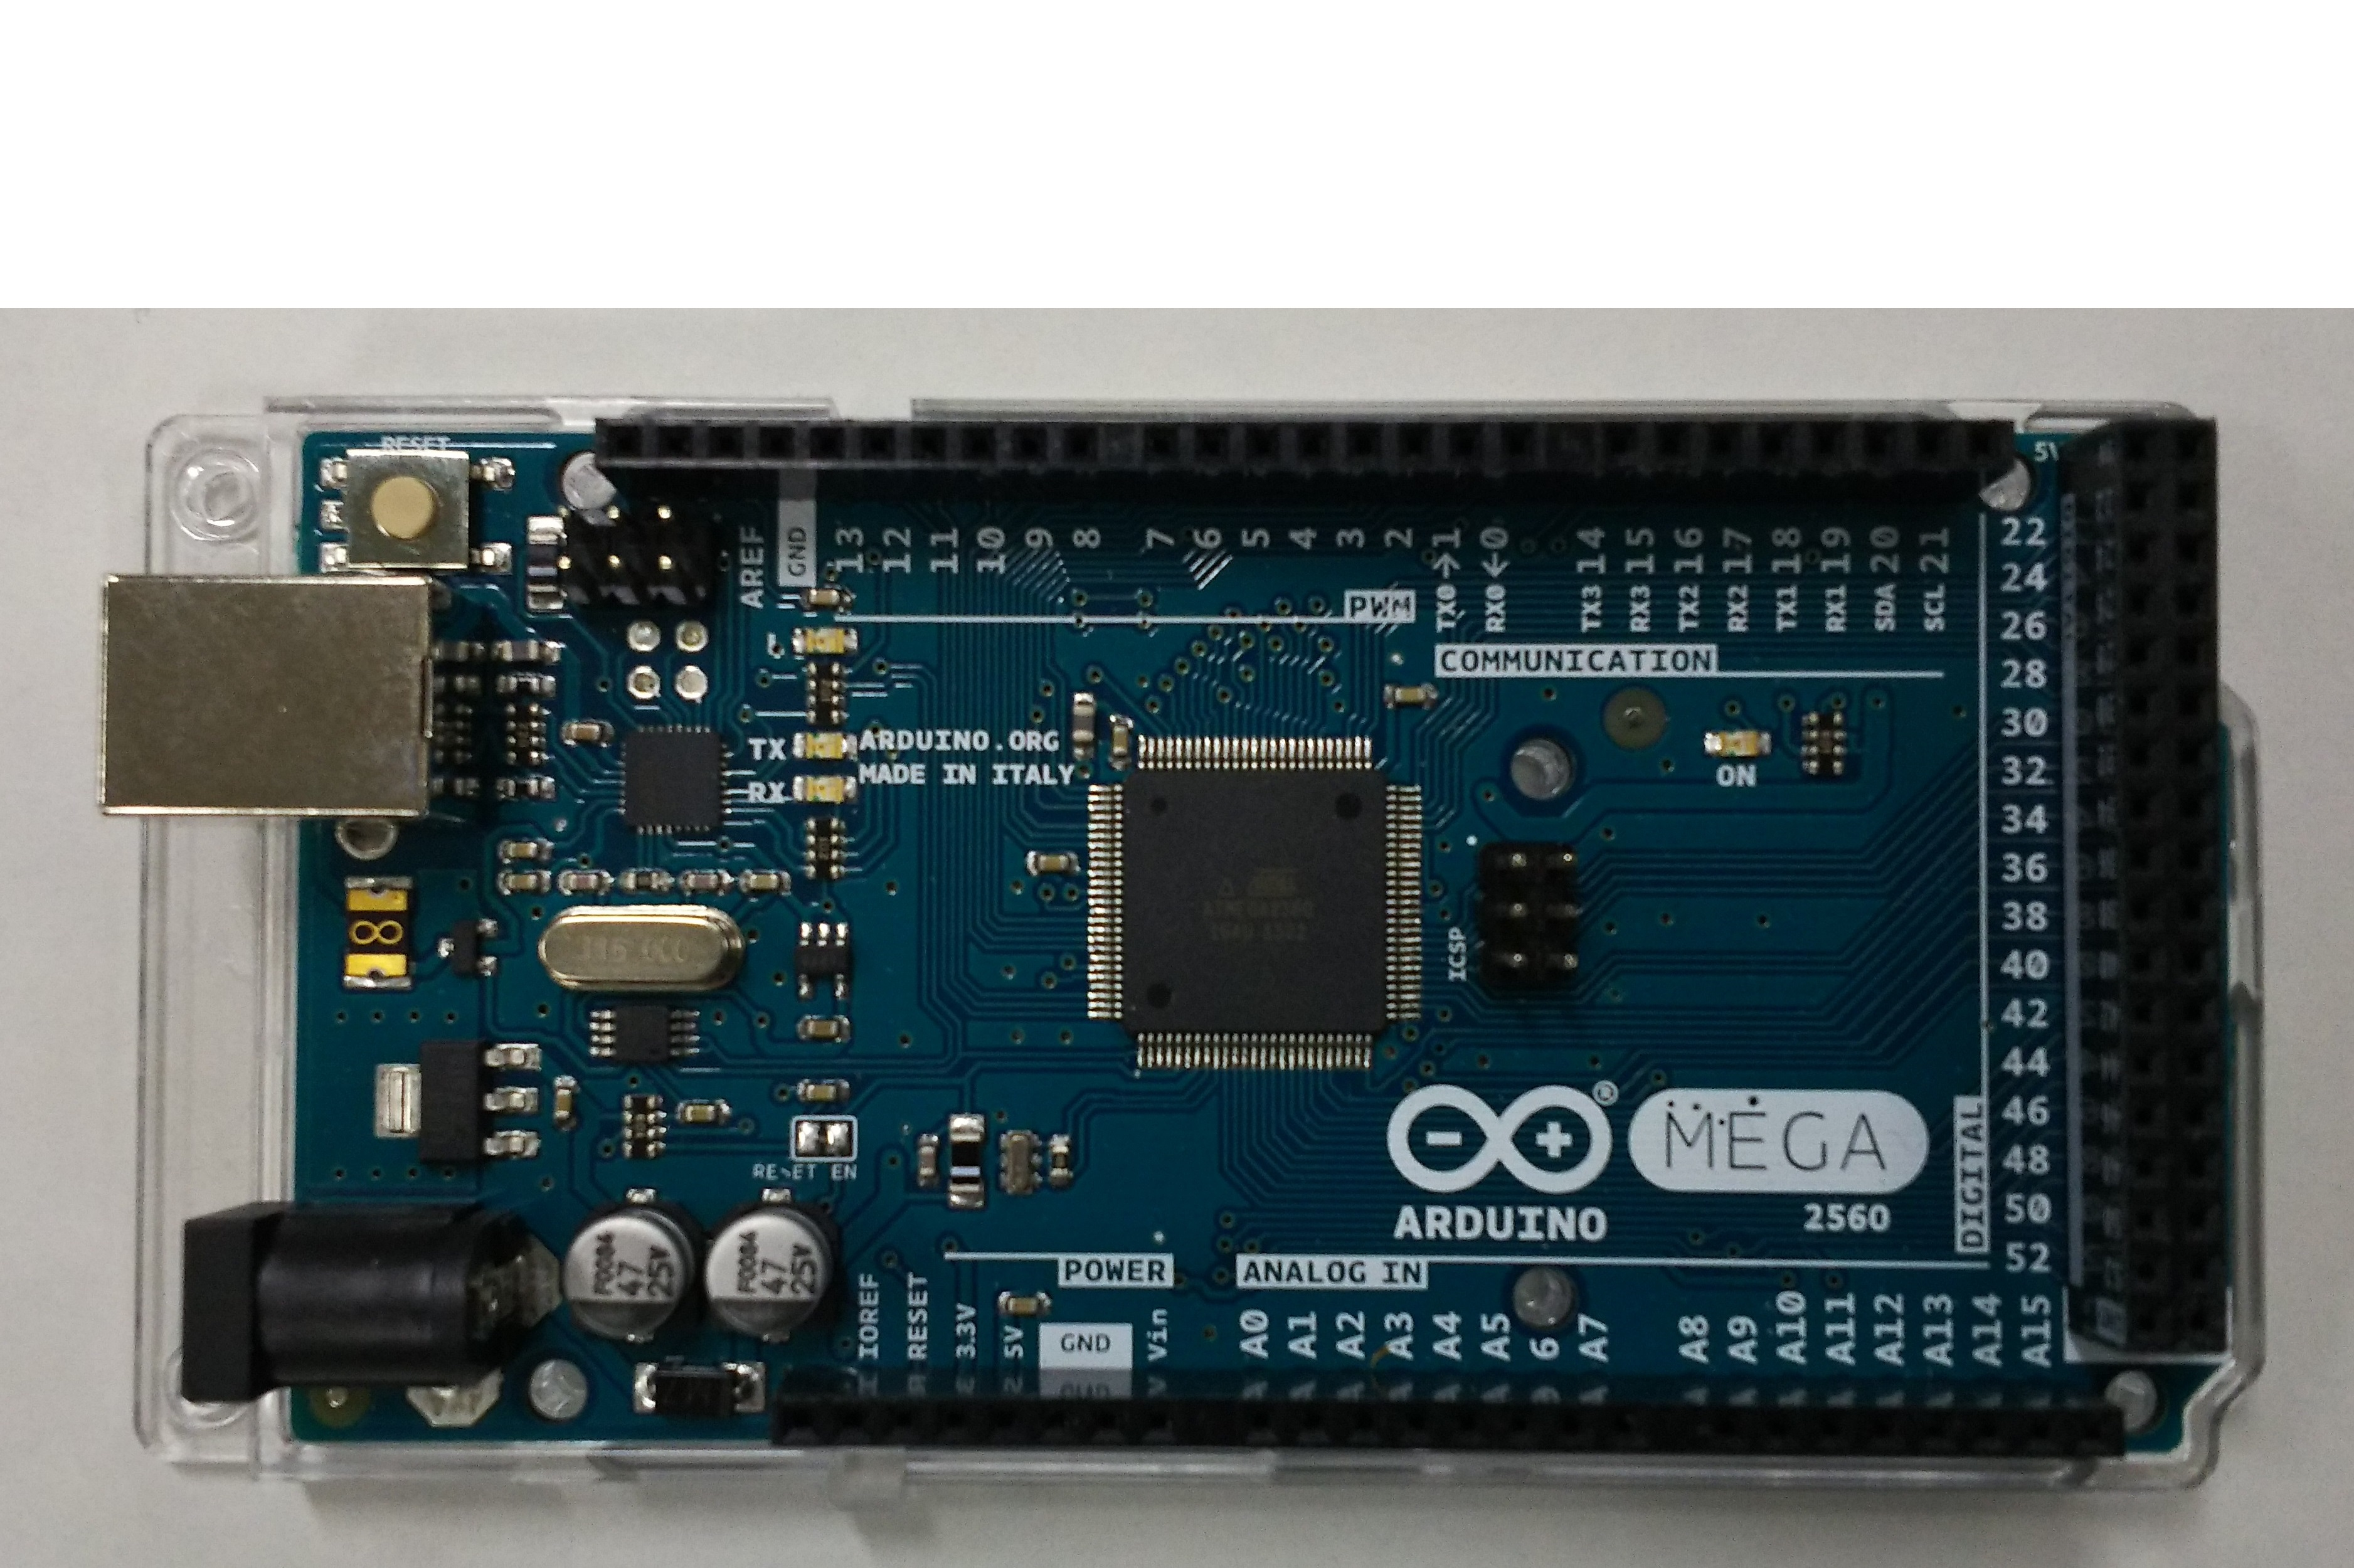
\includegraphics[width=100mm]{img/arduinoMega.JPG}
    \end{center}
  \caption{arduino Mega}
 \label{fig:arduino}
\end{figure}

\begin{figure}[htbp]
  \begin{center}
    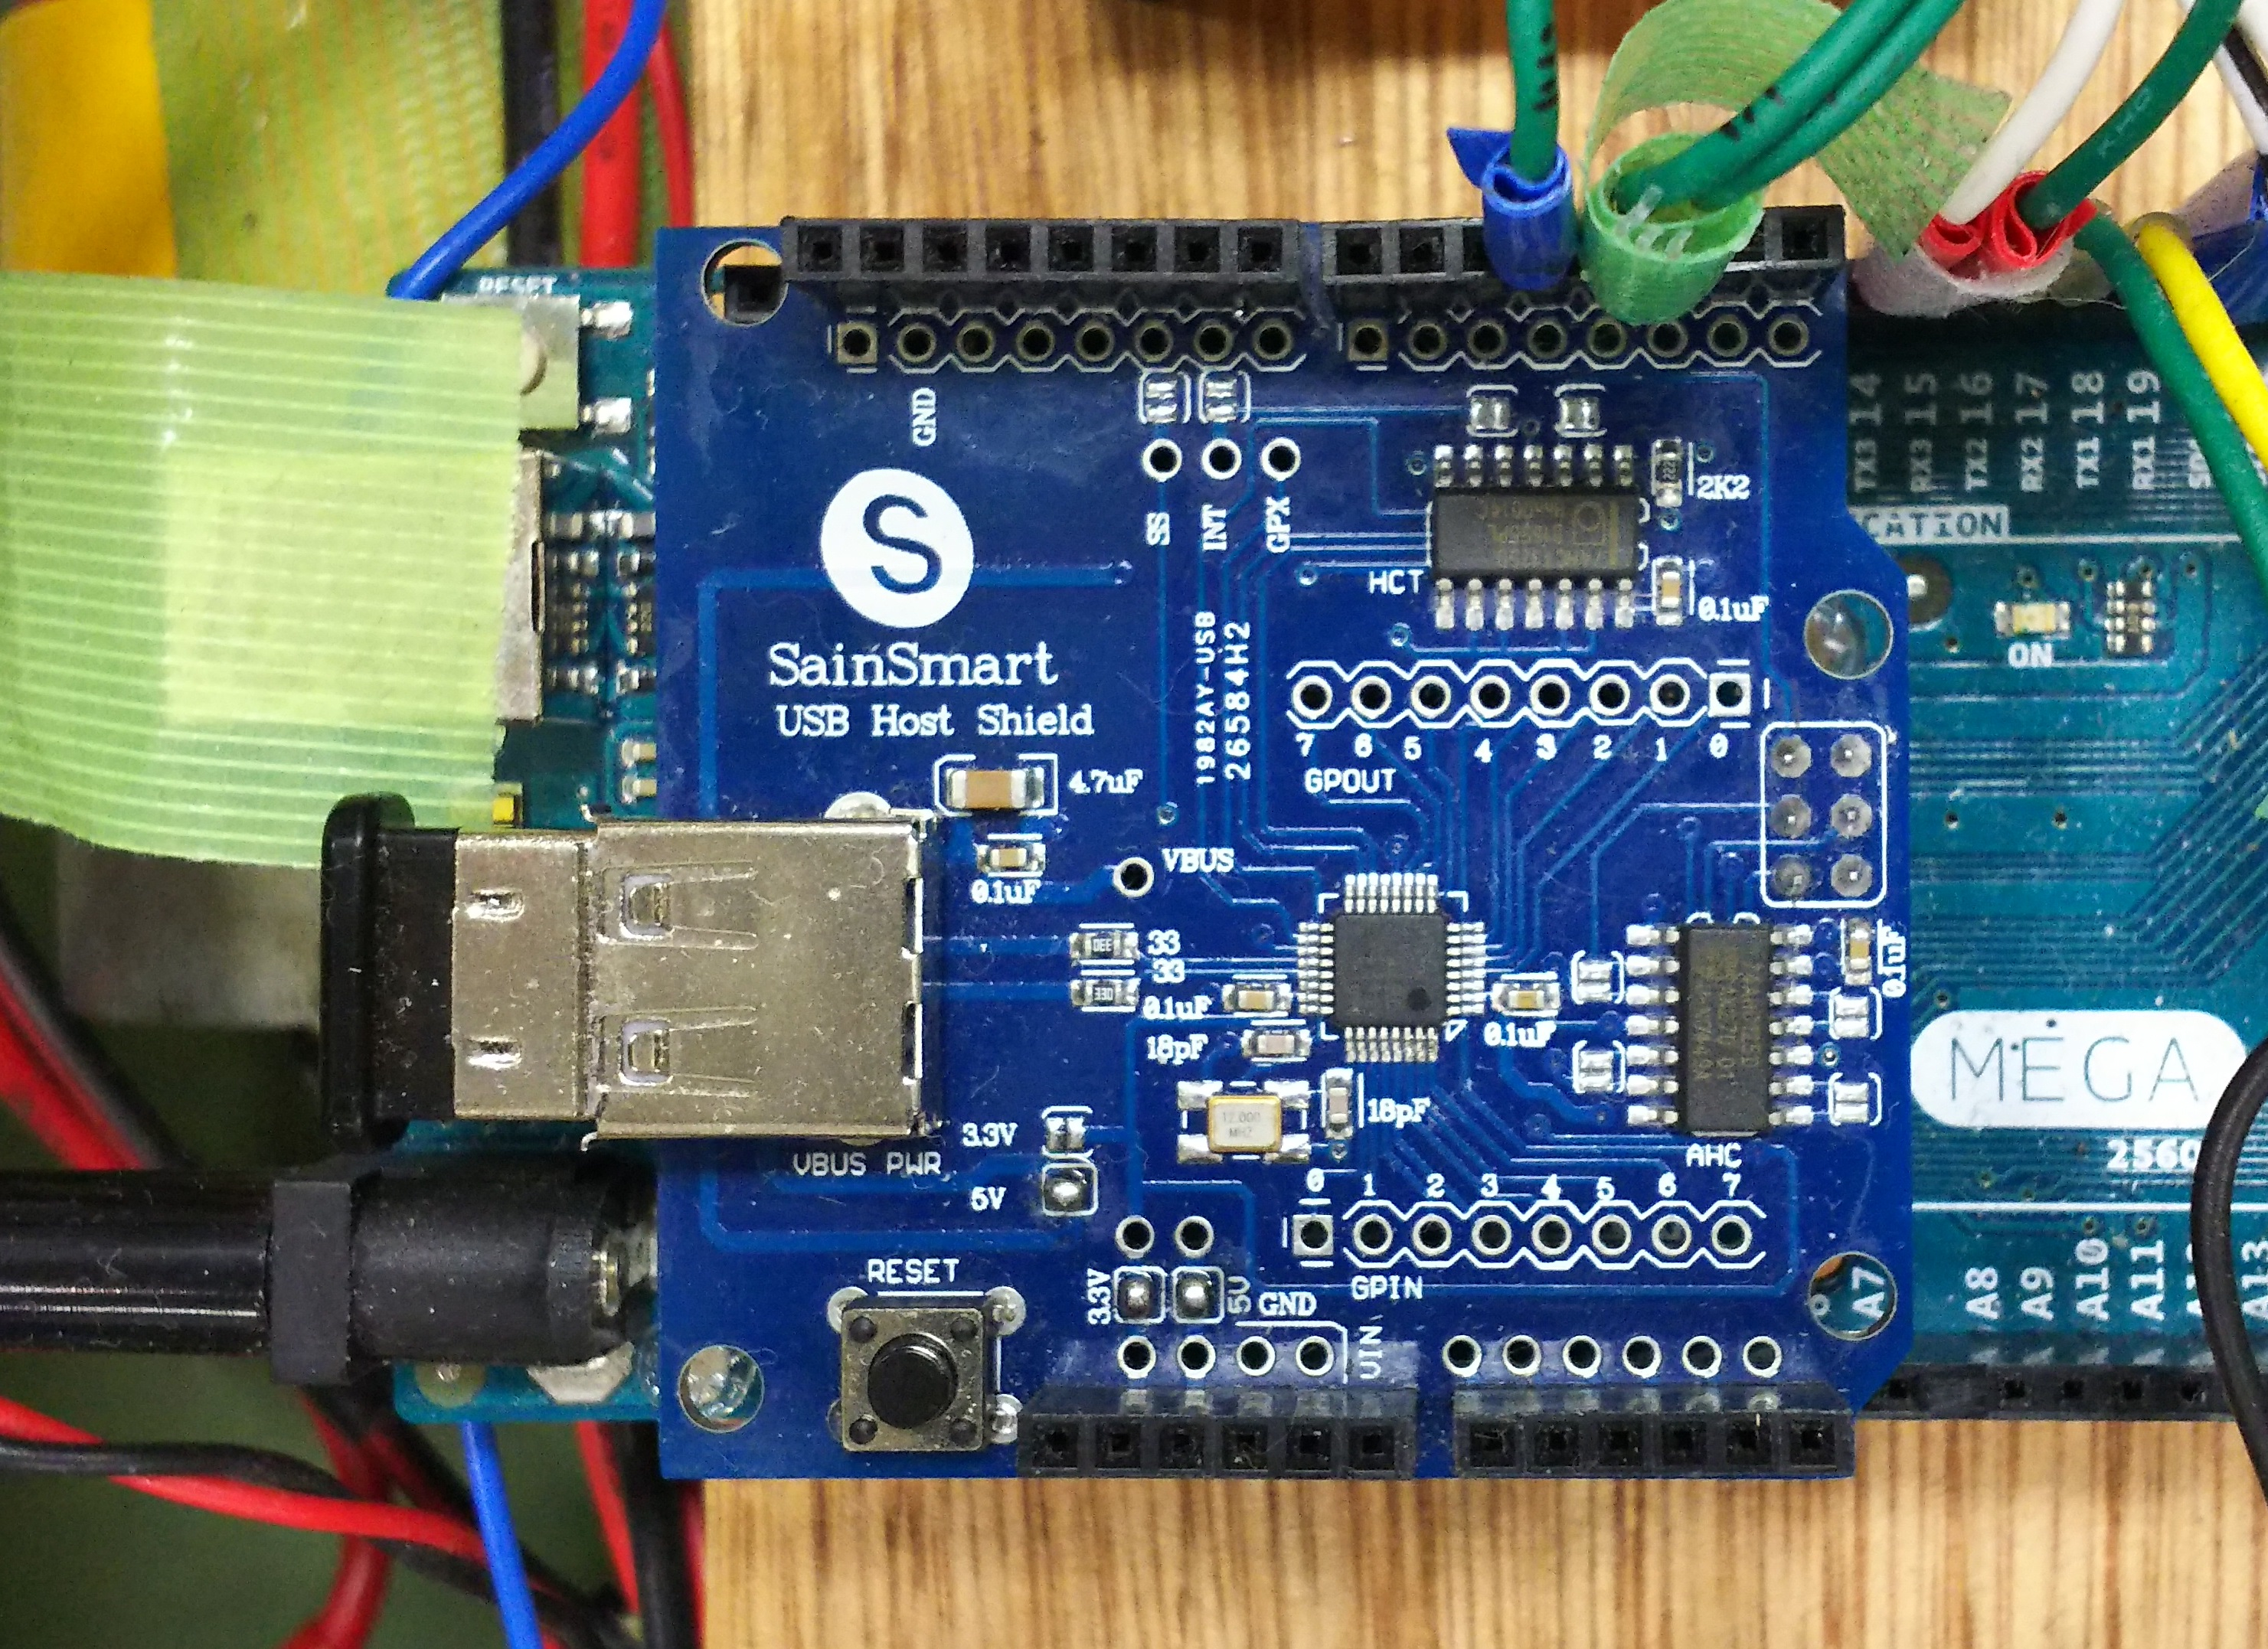
\includegraphics[width=100mm]{img/USBhs.JPG}
    \end{center}
  \caption{USBホストシールド}
 \label{fig:USBhs}
\end{figure}

\begin{figure}[!htbp]
  \begin{center}
    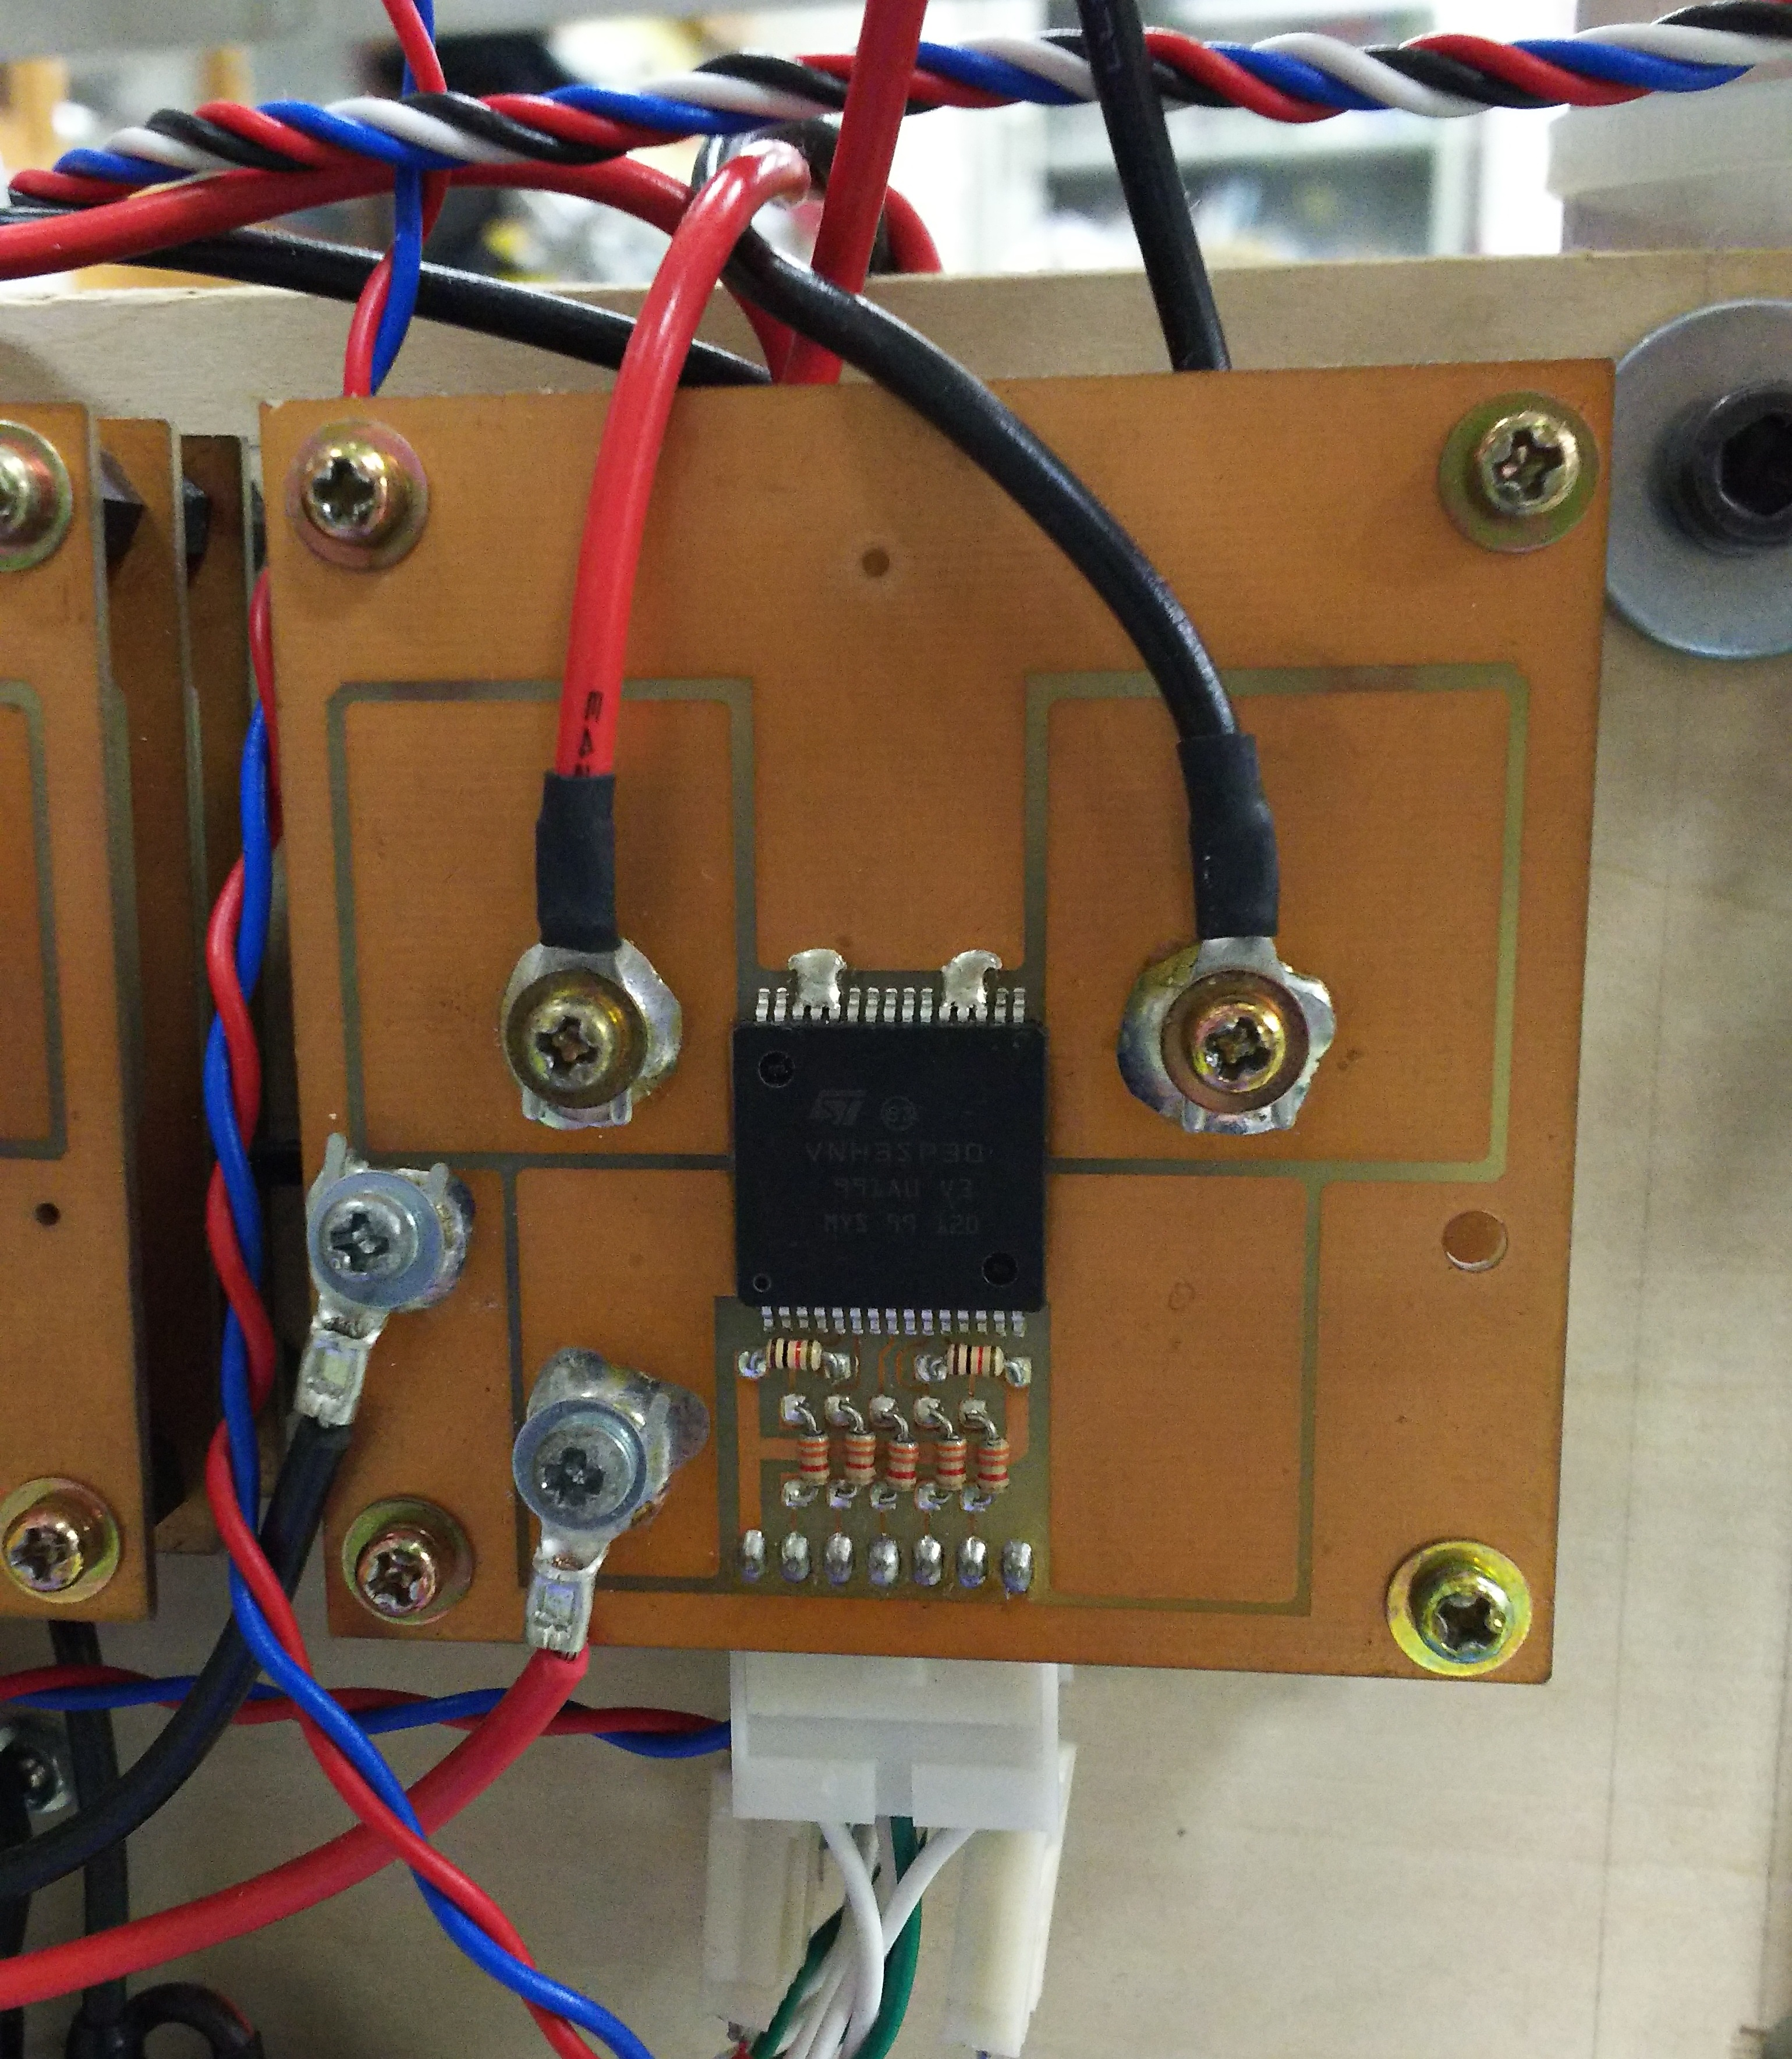
\includegraphics[width=90mm]{img/motordrive.JPG}
    \end{center}
  \caption{モータドライバ}
 \label{fig:motordrive}
\end{figure}

\section{使用部品}
使用した部品の詳細を以下の表\ref{tab:parts}に示す.

\begin{table}[!htb]
 \begin{center}
  \caption{搭載部品の型番とメーカ}
  \begin{tabular}[htbp]{|c|c|c|}
   \hline
   製品名&型番&メーカ \\
   \hline
   arduino&ArduinoMega&Arduino SRL\\
   \hline
   USBホストシールド&BOO6J4GOOO&サインスマート\\
   \hline
   DCモータ&組み合わせモータ323726&マクソン\\
   \hline
   コントローラ&DUALSHOCK3&ソニー\\
   \hline
   モータドライバ&-&夢考房\\
   \hline
   リミットセンサ&CNZ1023&パナソニック\\
   \hline
  \end{tabular}
  \label{tab:parts}
 \end{center}
\end{table}


\chapter{位置制御}位置制御とは,制御対象の現在位置を何らかのセンサなどで検出し,目標の位置になるようにフィードバック制御を行うことである.

\section{位置検出}例えばモータを動力とする位置制御をする際は,ロータリーエンコーダでモータの回転角度を検出することで制御対象の位置を特定する.このように,位置制御を行う際は位置を直接取得できるセンサを使用して,その値をフィードバックするのが一般的である.

\section{制御手法}
制御には主に以下のような手法が使われる.

\subsection{PID制御}目標値と現在値の差のことを偏差という.偏差に比例して制御量が増える制御を比例制御(P)といい,比例定数Kpは比例ゲインと呼ばれる.比例制御では偏差が0になると制御量が0になるため,いつまでたっても偏差が残り続ける事がある.この残留偏差をなくすため,偏差を時間で積分したものをKi倍して制御量に加えると,残留偏差のある時間が長いほど制御量が増えていき最終的に偏差が無くなる.これを積分制御(I)といい,Kiは積分ゲインと呼ばれる.偏差が急激な変化をする動き始めと動き終わりには,偏差を微分した値が大きくなる.微分に比例して制御量を大きくすると機敏な動作をするようになり,早く目標値に到達する.これを微分制御(D)といい,この比例定数Kdは微分ゲインと呼ばれる.これらP,I,D制御を組み合わせた基本的な制御手法がPID制御(図\ref{fig:PID})である.

\begin{figure}[htbp]
  \begin{center}
    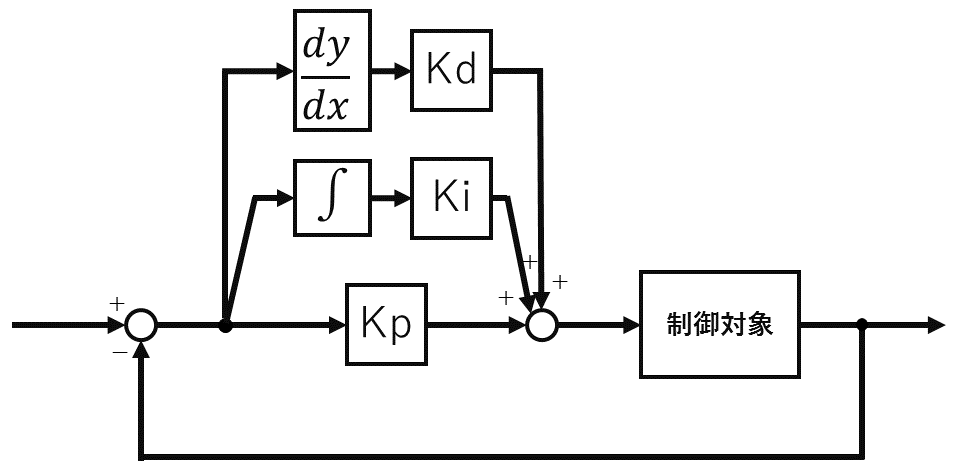
\includegraphics[width=120mm]{img/PID.png}
    \end{center}
  \caption{PID制御のブロック線図}
 \label{fig:PID}
\end{figure}

\subsection{極配置法}システムは式(\ref{eq:joutai})のような状態方程式という形で表すことが出来る.状態方程式はシステムへの入力$u$,システムからの出力$y$,システムの状態量$x$の関係を表した方程式である.システムは極と呼ばれる固有の値を持っており,その値によって応答速度や行き過ぎ量などの特性が変化する.状態方程式で表されたシステムに対し,状態量$x$に一定の値(ゲイン)を掛けて入力にフィードバックすることで極を変化させることができる.極を望ましい値に設定するフィードバックゲインを探る方法を極配置法という.

\begin{eqnarray}
\begin{array}{l}
\dot{x}=\bm{A}x+\bm{B}u\\
y=\bm{C}x+\bm{D}u
\end{array}
\label{eq:joutai}
\end{eqnarray}


\chapter{位置センサレス位置制御}

\section{センサレスの有効性}上述したように今回のリフトのような位置制御を行う場合,通常,モータの回転角度を検出するロータリーエンコーダを使用して移動量を算出する.しかし,ロータリーエンコーダを使用するにはそれ専用の取付部を新しく設計し取り付けるか,既にロータリーエンコーダと一体化しているモータを購入し使用する必要がある.ロータリーエンコーダを取り付けるにはブラケットや軸継手が必要になり,さらに取付精度も要求される.一体化されたモータなら精度は確保されているが,一般に高価である.
このように,ロータリーエンコーダを後から取り付ける場合は金銭的,時間的にコストがかかる場合が多い.今回提案する位置制御はロボットに取り付ける専用のパーツを使わないため,実現できればそれらのコストを減らすことができる.

\section{センサレス制御の方法}
モータの電流,電圧,回転速度には相関があり,二つの値が定まると残りの一つの値も定まる.電圧の値は操作量なので既知であるため,電流の値が取得できれば,モータの回転速度を求め,それを積分して回転角度を求め,そこから移動量を算出することが出来る.必要なものは電流センサを使った電流計測回路のみなので,ロータリーエンコーダを使うよりも後付けを簡単に行うことができる.

\subsection{制御対象のモデル}
リフトの簡略モデルを図\ref{fig:liftModel}に示す.リフトの運動方程式は式(\ref{eq:lift})のようになる.

\begin{figure}[htbp]
  \begin{center}
    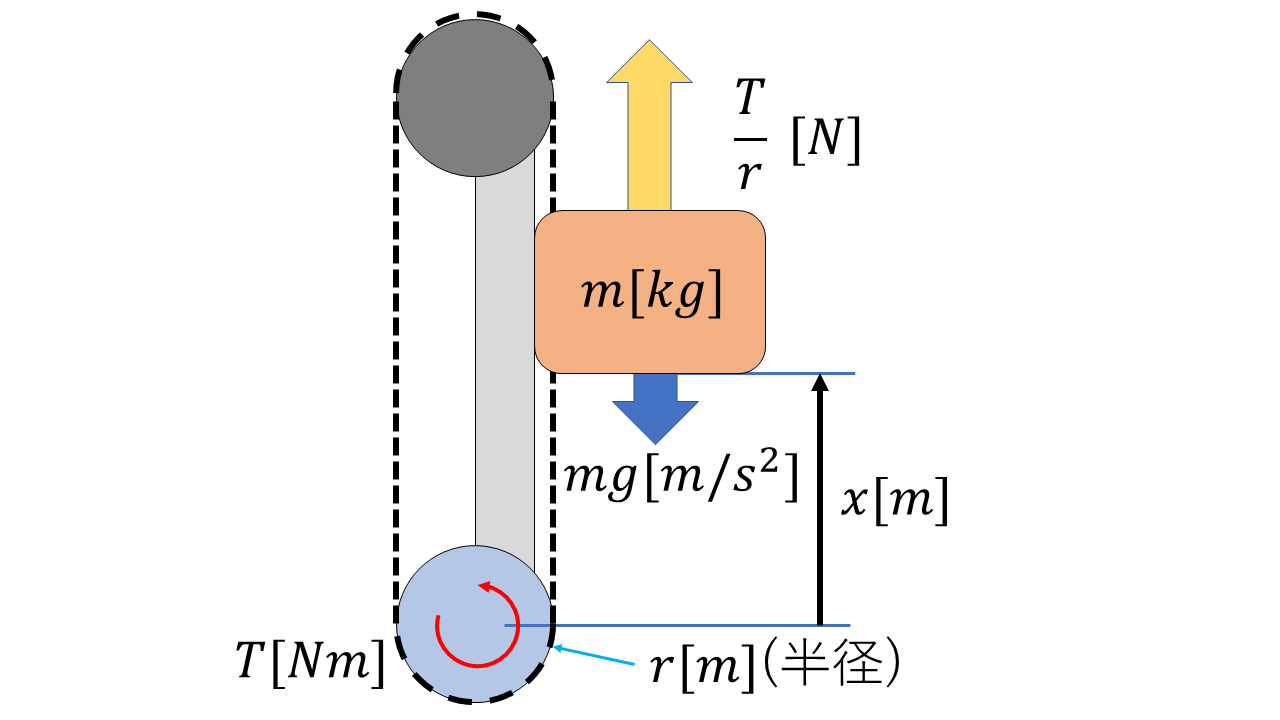
\includegraphics[width=170mm]{img/liftModel.png}
    \end{center}
  \caption{リフトの簡略モデル}
 \label{fig:liftModel}
\end{figure}

\begin{eqnarray}
m\dot{v}=\frac{T}{r}-mg\\
\label{eq:lift}
\end{eqnarray}

式(\ref{eq:lift})をトルクについて変形すると,式(\ref{eq:lift2})のようになる.

\begin{eqnarray}
T=rm(\dot{v}+g)\\
\label{eq:lift2}
\end{eqnarray}

モータ回路の簡略モデルを図\ref{fig:circuitModel}に示す.モータの運動方程式は式(\ref{eq:motor})のようになる.

\begin{figure}[htbp]
  \begin{center}
    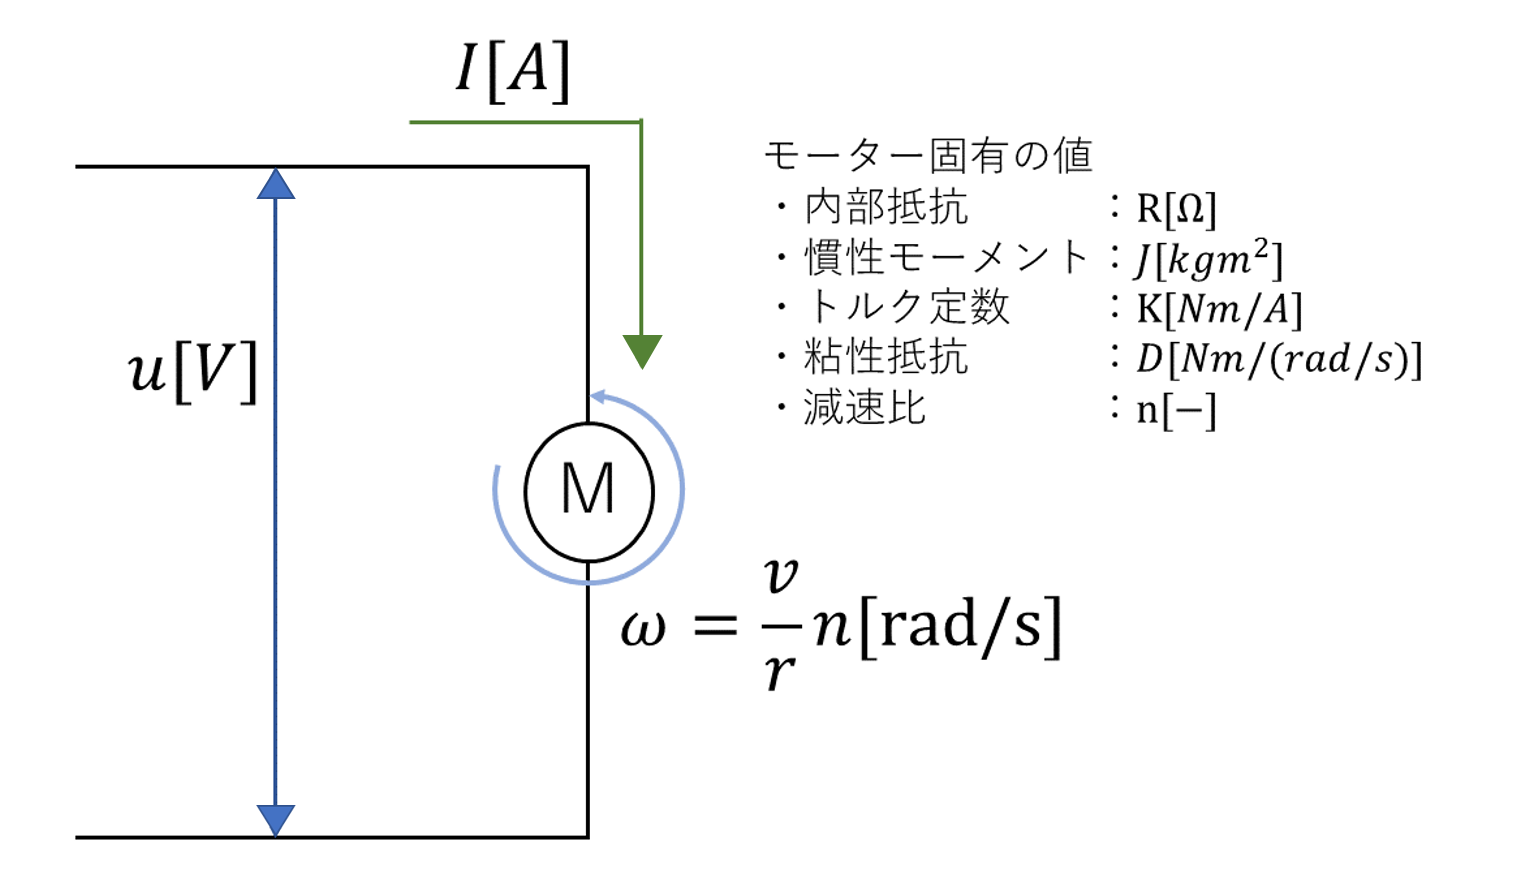
\includegraphics[width=150mm]{img/circuitmodel.png}
    \end{center}
  \caption{モータ回路簡略モデル}
 \label{fig:circuitmodel}
\end{figure}

\begin{eqnarray}
RI+K{\omega}=c\\
J\dot{\omega}+\frac{D}{n}{\omega}-\frac{T}{n}=KI
\label{eq:motor}
\end{eqnarray}

モータの回転数と歯車比,スプロケット半径との関係は式(\ref{eq:rote-v})で表される.

\begin{eqnarray}
{\omega}=\frac{v}{n}r
\label{eq:rote-v}
\end{eqnarray}

リフトの上昇速度を状態量に,電流値を観測方程式とする状態方程式を立てる.式(\ref{eq:lift}),式(\ref{eq:motor})より,リフトの状態方程式は式(\ref{eq:system})のようになる.

\begin{eqnarray}
%\begin{array}{l}
\dot{v}=-\frac{RD+K^2}{RJ+r^{2}m/n^2}v+\frac{KRn}{RJn^{2}+r^{2}m}u-\frac{g}{Jn^{2}/r^{2}m+1}\\
I=-\frac{Kn}{Rr}v+\frac{1}{R}u
%\end{array}
\label{eq:system}
\end{eqnarray}


\subsection{制御系設計}ブロック線図を図\ref{fig:blocksenzu}に示す.

\begin{figure}[htbp]
  \begin{center}
    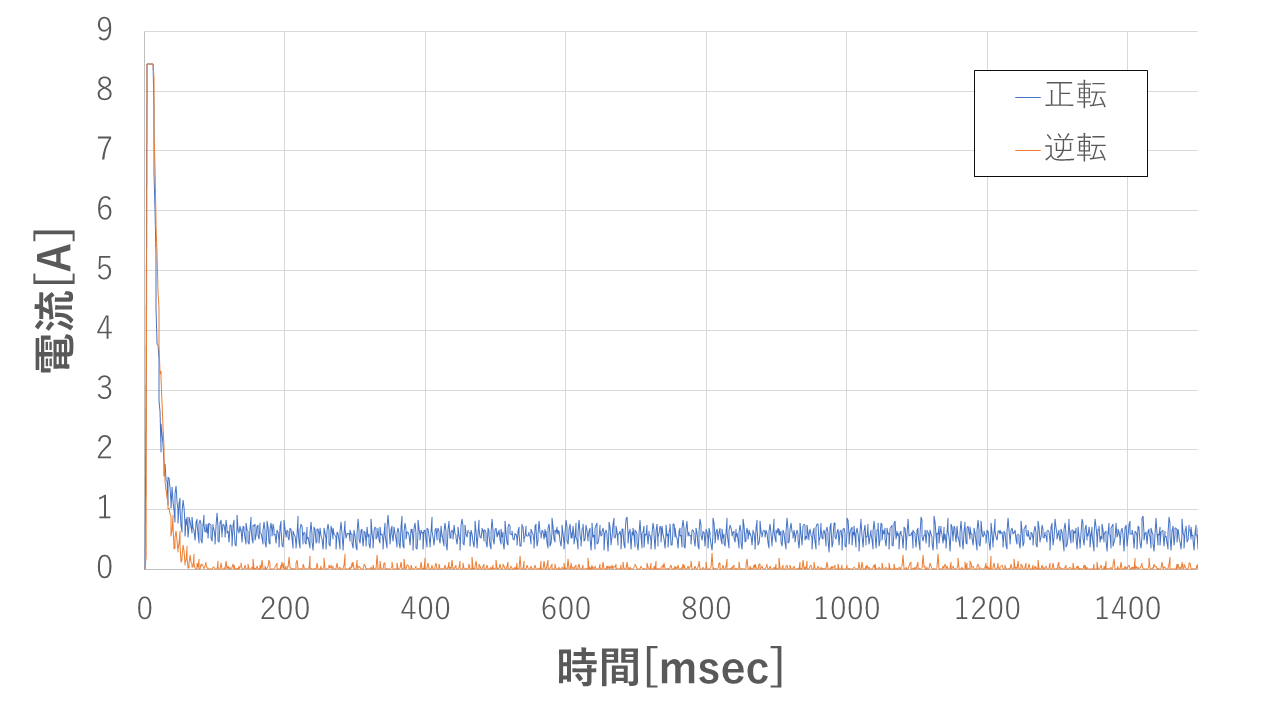
\includegraphics[width=130mm]{img/blocksenzu.png}
    \end{center}
  \caption{ブロック線図}
 \label{fig:blocksenzu}
\end{figure}

リフトには,目標値と現在値の偏差に比例した値を入力する比例制御を行っている.通常の位置制御であればリフトの位置を直接検出してフィードバック制御を行う.しかし今回のセンサレス制御では位置を検出できない.そのため,電流センサから得た電流と入力の電圧から速度測定器でリフトの移動速度を求め,それを積分した値を現在値としてフィードバックする.速度推定器は式(\ref{eq:speed})で表される.

\begin{eqnarray}
v=-\frac{Rr}{Kn}i+\frac{R^2r}{Kn}u
\label{eq:speed}
\end{eqnarray}

速度測定器で算出した移動速度は実際のリフトの移動速度とは異なる可能性がある.


\chapter{実験}
\section{シミュレーション}
シュミレーションを利用して,設計した制御系の性能を確認する.

\subsubsection{シミュレーションソフト}
シミュレーションには数値計算ソフト「Scilab」に付属しているビジュアルモデリングソフト「Xcos」を使用する.Xcosで組み立てたブロック線図を図\ref{fig:blockXcos}に示す.この際、リフトにかかる電圧の絶対値の最大は実際と同じく12[v]に制限した.

\begin{figure}[htbp]
  \begin{center}
    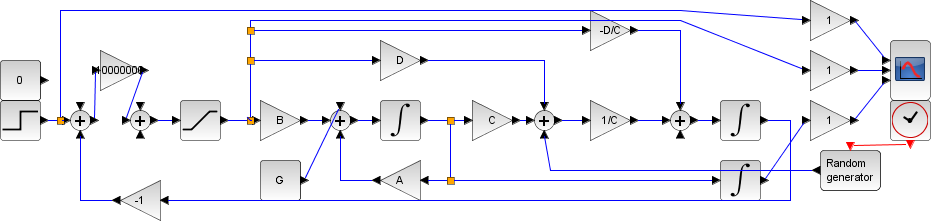
\includegraphics[width=150mm]{img/blockXcos.png}
    \end{center}
  \caption{Xcosで組み立てたブロック線図}
 \label{fig:blockXcos}
\end{figure}

\subsubsection{シミュレーション結果}
シミュレーションの結果を図\ref{fig:sim}に示す.

\begin{figure}[htbp]
 \begin{center}
    \includegraphics[width=150mm]{img/sim.bmp}
    \end{center}
  \caption{入力した目標値による電圧と位置の時間変化}
 \label{fig:sim}
\end{figure}

\subsubsection{測定誤差の影響}
実際に電流を測定した時には誤差があると考え,誤差の影響を見るため電流の値を分散が1[A]の正規分布になるようにした.その際のシミュレーション結果を図\ref{fig:sim}に示す.

\begin{figure}[htbp]
 \begin{center}
    \includegraphics[width=150mm]{img/sim2.bmp}
    \end{center}
  \caption{入力した目標値による電圧と位置の時間変化}
 \label{fig:sim}
\end{figure}

電圧のグラフが激しく振動している為,塗りつぶされて見える.これは電流のノイズの影響だと考えられるが,ノイズの平均値が0ならば現在位置に影響はなかった.

\section{検出誤差の確認}
電流センサが検出する電流と実際に流れている電流に誤差があると,リフトの速度推定にも誤差が生じてしまい,時間がたつにつれリフトの位置がずれていってしまう.ここでは電流センサで検出した値がどれだけの測定誤差を持つのか確認する.

\subsubsection{使用機器}
モータドライバは電流センサを内蔵したものを使用した.使用したモータドライバを図\ref{fig:currentDriver}に示す.使用した機器一覧を表\ref{tab:partsCurrent}に示す.

\begin{figure}[htbp]
 \begin{center}
    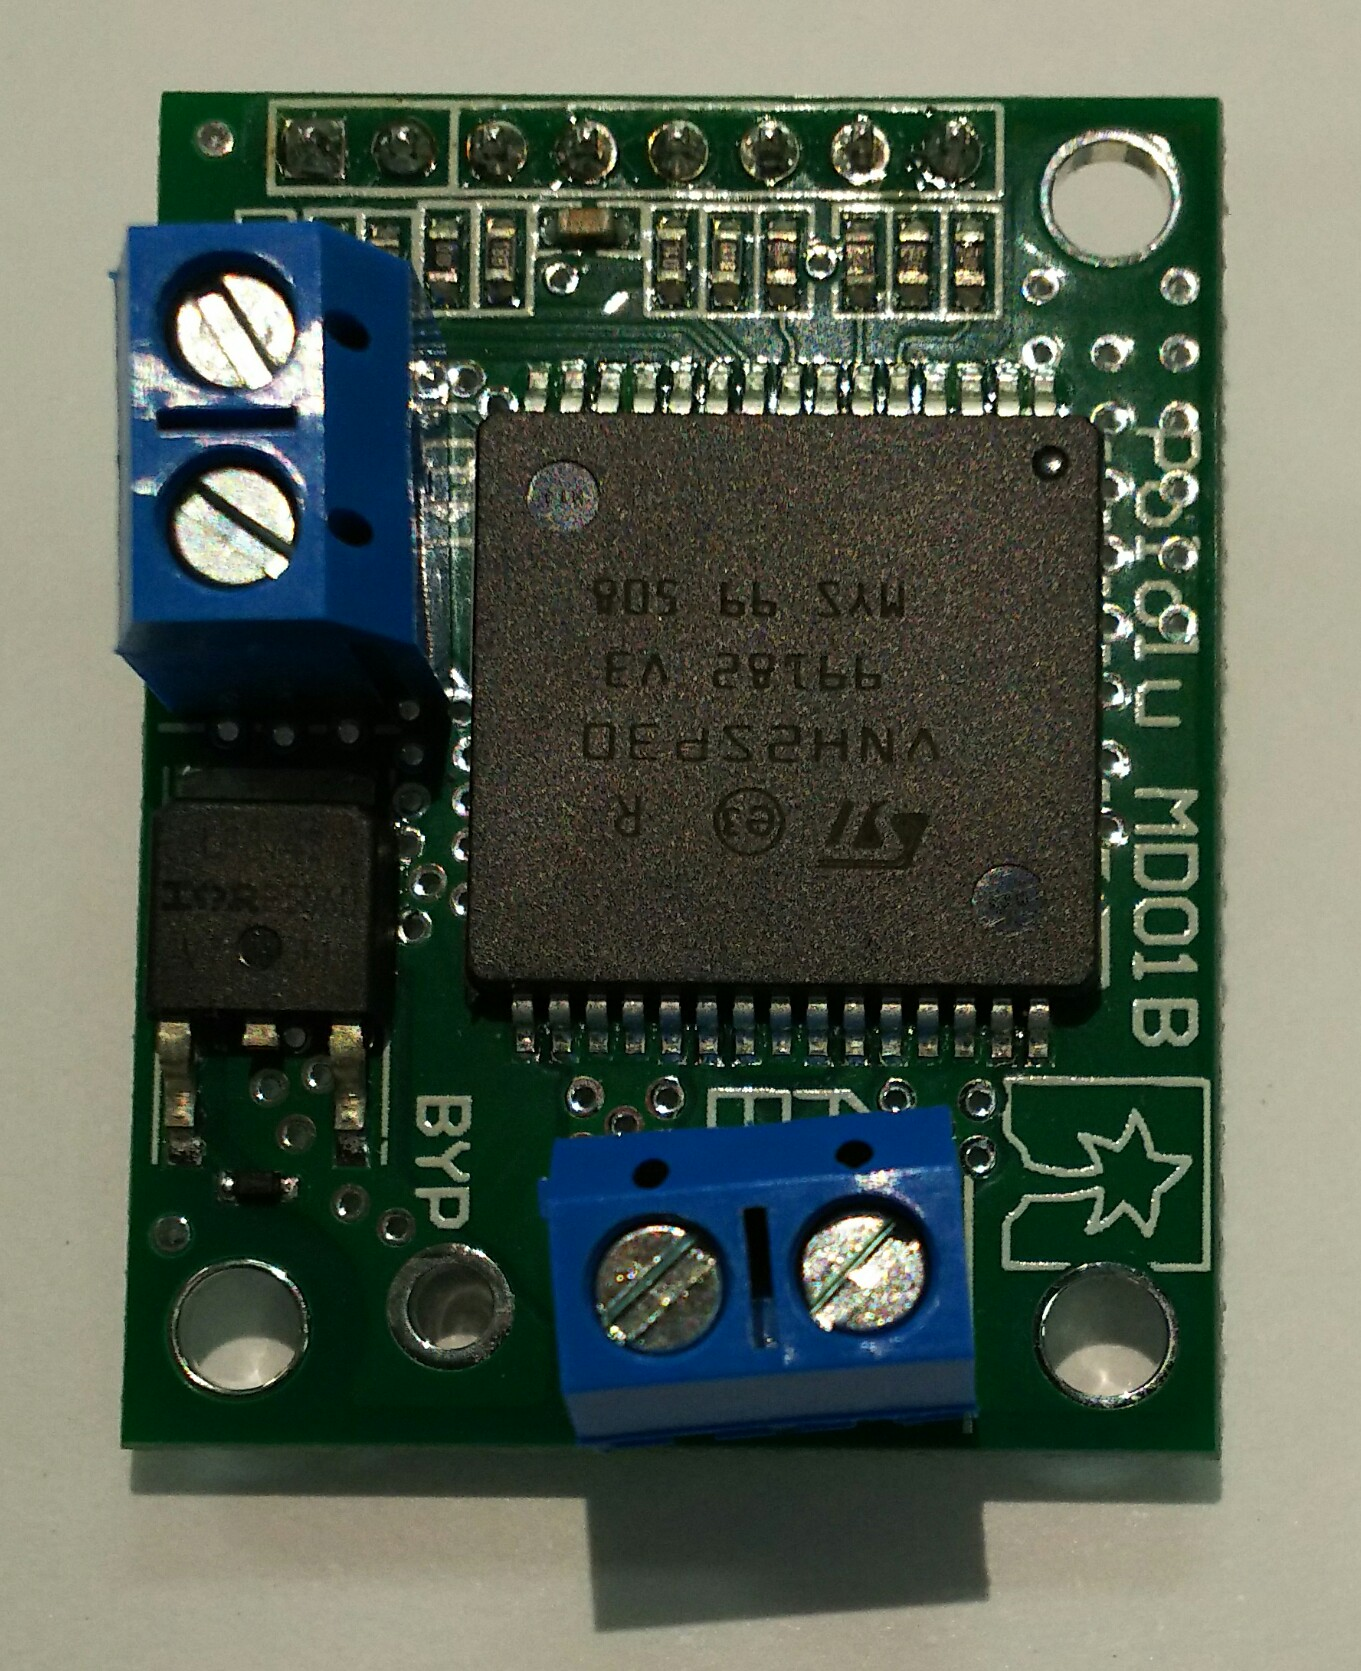
\includegraphics[width=75mm]{img/currentDriver.JPG}
    \end{center}
  \caption{電流センサ内臓モータドライバ}
 \label{fig:currentDriver}
\end{figure}

\begin{table}[htb]
 \begin{center}
  \caption{搭載部品の型番とメーカ}
  \begin{tabular}[htbp]{|c|c|c|}
   \hline
   製品名&型番&メーカ \\
   \hline
   arduino&ArduinoUno&Arduino SRL\\
   \hline
   DCモータ&組み合わせモータ323726&マクソン\\
   \hline
   電流センサ内臓モータドライバ&MD01B&Pololu\\
   \hline
   テスター&VOAC86&IWATU\\
   \hline
  \end{tabular}
  \label{tab:partsCurrent}
 \end{center}
\end{table}

\subsubsection{計測方法}
モータに電圧を12[v]印加し.電流センサから値を1ミリ秒ごとに記録し,平均とノイズの分散を算出する.その後,テスターで実際の電流を計測し,電流センサで得た平均値との差をノイズの平均値とする.

\subsubsection{電流計測}
電流を計測した結果を図\ref{fig:currentMeasurement}に示す.

\begin{figure}[htbp]
 \begin{center}
    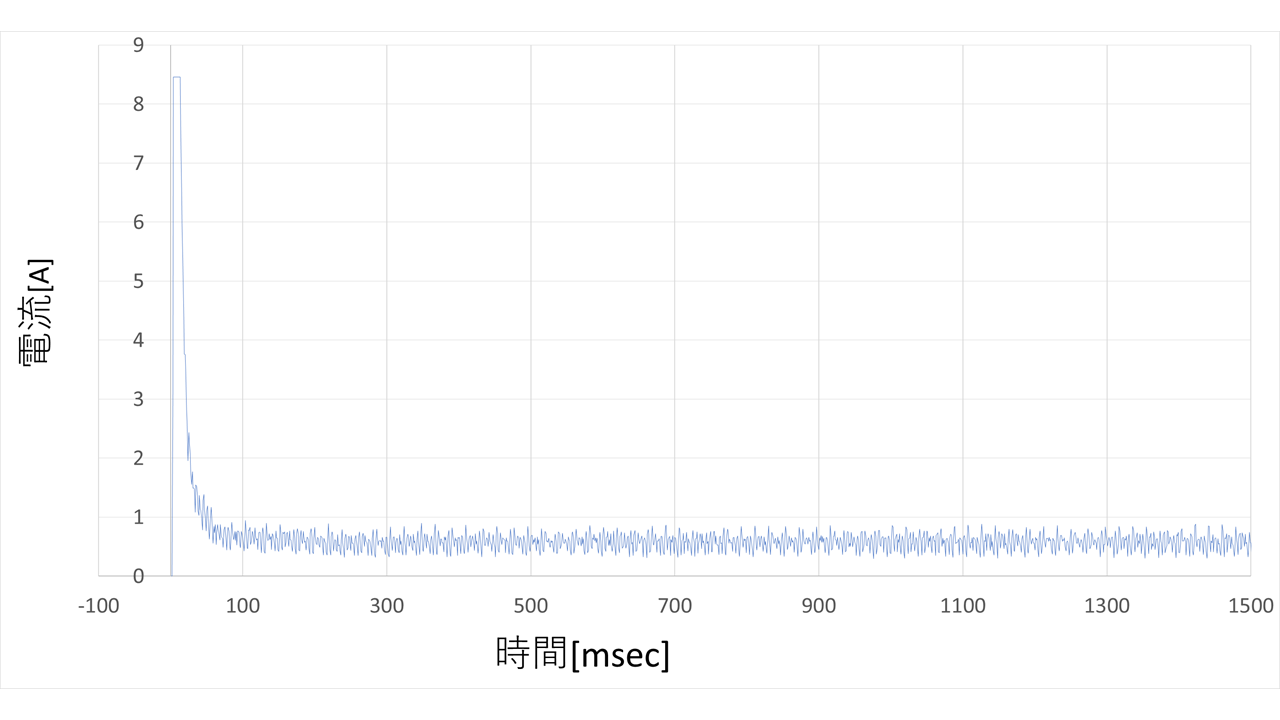
\includegraphics[width=150mm]{img/currentMeasurement.png}
    \end{center}
  \caption{電流の時間変化}
 \label{fig:currentMeasurement}
\end{figure}

平均は0.575[A],ノイズの分散は1.880[A],テスターでの計測結果は0.232[A]となった.よってノイズの平均は0.343[A]となった.


\chapter{おわりに}シミュレーションを使用して,センサレス制御は可能であることを確認することができた.この制御を実際のリフトに適用する際には,モータのモデル化誤差と電流センサのノイズによって引き起こされる速度推定誤差を何らかの方法で補正するなどして解決する必要があると考えられる.

\begin{thebibliography}{8}
\bibitem{ob} 熊谷正朗,状態フィードバックとオブザーバ,www.mech.tohoku-gakuin.ac.jp\slash{}rde\slash{}contents\slash{}course\slash{}controlII\slash{}statefeedback.html,2011\slash{}02\slash{}10
\bibitem{sei} 明石 一・今井弘之,制御工学演習,共立出版,2014\slash{}04\slash{}15
\end{thebibliography}







\chapter*{謝辞}
\addcontentsline{toc}{chapter}{謝辞}
本論文作成にあたり研究の考え方,方法のまとめ方など長期にわたって熱意のあるご指導,ご鞭撻していただいた,伊藤恒平教授に厚く御礼申し上げます.

特に制御においても論文の書き方においても論文を何度も読んでいただき,指導していただいた伊藤恒平教授,伊勢大成講師に大変ご苦労をかけてしまいましたことにも心よりお詫び申し上げます.

その他,助けていただいた多くの皆様に心から感謝しております.ありがとうございました.

\appendix
\chapter{プログラム}

\lstinputlisting[caption=電流計測プログラム(Arduino Uno),label=program]{program_Keisoku.cpp}




\end{document}






